\documentclass[conference,10pt,letterpaper]{IEEEtran}
\usepackage[T1]{fontenc}
\usepackage[utf8]{inputenc}
\usepackage{amsmath,amssymb,booktabs,graphicx,adjustbox,array}
\usepackage{xurl}
\usepackage[hidelinks]{hyperref}
\hypersetup{pdftitle={Evidence Acquisition and Output Reliability for Advisory-Guided Vulnerability Localization},pdfkeywords={vulnerability localization, evidence acquisition, output reliability}}
% Generated numbers; no fitted changes to inference.
\newcommand{\SOnePrimary}{0.3250}
\newcommand{\SOnePrimaryCI}{[0.2271, 0.4229]}
\newcommand{\SOneAgentRagFR}{-0.0250}
\newcommand{\SOneAgentRagFRP}{0.3970}
\newcommand{\SOneAgentRagLR}{0.0875}
\newcommand{\SOneAgentRagLRQ}{0.0149}
\newcommand{\SOneInputRatio}{10.57}
\newcommand{\SOneFee}{47.243}
\newcommand{\SOneAllFee}{47.304}
\newcommand{\SOneFailureInvalid}{22}
\newcommand{\SOneFailureEmpty}{9}
\newcommand{\SOneLocoMin}{0.2894}
\newcommand{\SOneLocoMax}{0.3377}
\newcommand{\SOneRepoEqual}{0.2228}
\newcommand{\SOneAgentFR}{0.7479}
\newcommand{\SOneAgentLR}{0.5813}
\newcommand{\SOneRagFR}{0.7729}
\newcommand{\SOneRagLR}{0.4938}
\newcommand{\SOnePackFR}{0.4229}
\newcommand{\SOnePackLR}{0.2500}
\newcommand{\SOneCompletionOpenN}{187}
\newcommand{\SOneCompletionOpenValid}{187}
\newcommand{\SOneCompletionOpenDsml}{0}
\newcommand{\SOneCompletionOpenEmpty}{0}
\newcommand{\SOneCompletionClosedN}{53}
\newcommand{\SOneCompletionClosedValid}{22}
\newcommand{\SOneCompletionClosedDsml}{22}
\newcommand{\SOneCompletionClosedEmpty}{9}

\title{Evidence Acquisition and Output Reliability for\\Advisory-Guided Vulnerability Localization}
\author{\IEEEauthorblockN{Authors to be specified}}
\begin{document}
\maketitle
\begin{abstract}
We compare read-only adaptive exploration, single-round hybrid retrieval, and lexicographic packing for advisory-guided vulnerability localization using DeepSeek V4 Pro and a 50,000-token repository-information ceiling. Two separately reported studies each contain 720 outcomes on the same 80 VulnGym entries from 13 repositories. Inputs include dataset-supplied titles; 47 contain target filenames. In the supplementary study with shared nonblank source eligibility, exploration delivers annotated code for 91.25\% of entry-point and critical-operation opportunities, versus retrieval's 38.13\%, but mean file recall is 0.7479 versus 0.7729. Joint analysis qualifies this contrast: 80 of exploration's 108 uncovered annotations with source available are entry points, although the task does not explicitly request both annotation roles. Retrieval earns 96 interval hits without the corresponding annotated source, but only five remain when predictions are limited to 64 lines. Schema-valid answers also contain nonexistent paths and out-of-bounds intervals. All 31 exploration output failures remain scored zero; their contribution to the file-recall contrast offsets the positive contribution from other paired outcomes. Exploration returns narrower intervals and higher tolerance-based interval recall, with inferential support sensitive to repository dependence, while consuming 10.57 times packing's cumulative provider input. The results distinguish source availability, annotation coverage, interval extent, and output validity within these configurations. They motivate reporting these dimensions together when evaluating title-assisted localization.
\end{abstract}
\begin{IEEEkeywords}
vulnerability localization, repository context, coding agents, retrieval-augmented generation, empirical evaluation
\end{IEEEkeywords}
\section{Introduction}
An advisory can describe an authorization bypass or unsafe operation without identifying the responsible source lines. Locating those lines requires navigating a repository, often across an externally reachable entry point and a security-critical operation. A language model can use advisory clues, repository evidence, and prior knowledge to propose those locations. This acquisition can be task-independent, driven by a retrieval query, or adapted through successive tool interactions.

The comparison is more involved than assigning each method the same context limit. A file may be eligible for a method but never selected; a selected span may contain little relevant evidence; and an informative interaction may still end without a usable answer. Replaying an interactive history also consumes provider input without delivering new repository information. Consequently, localization recall alone cannot establish either acquisition effectiveness or resource efficiency.

We examine these distinctions through three implemented configurations for advisory-guided localization: a read-only exploration Agent, single-round hybrid retrieval (RAG), and lexicographic context packing (Pack). All use DeepSeek V4 Pro and a 50,000-token ceiling on the repository-information ledger. Inputs combine a VulnGym entry title with a truncated public advisory description. Entry titles can include filenames appended during dataset annotation; 47 of the 80 supplied titles contain an EP/CO target basename. We therefore study localization with these dataset-supplied titles, rather than assuming an unmodified advisory input. Explicit entry-point (EP) and critical-operation (CO) annotation fields are supplied to the evaluator, while their filename clues may also occur in input text~\cite{vulngym,vulngymdata}. The model predicts up to five file/line intervals; the task concerns known vulnerabilities.

Three research questions organize the study:
\begin{itemize}
\item \textbf{RQ1:} How do the complete configurations differ in file and line recall when every scheduled model outcome is retained?
\item \textbf{RQ2:} How do source delivery, EP/CO annotation coverage, prediction extent, and output validity co-occur?
\item \textbf{RQ3:} What delivered information, cumulative provider input, reported fees, and online execution time accompany these outcomes?
\end{itemize}

The evidence consists of an original study (S0) and a supplementary study (S1), each comprising 720 outcomes: 80 advisory-distinct entries, three configurations, and three repeats. S1 reuses the known sample after S0 inspection and jointly revises source eligibility, indexing, code presentation, and the Agent interface. We preserve both studies and report them separately. S1 supplies a comparison with shared nonblank source eligibility; it is neither an independent-sample confirmation nor an ablation of a single change.

Our contribution is an empirical characterization of how the interpretation of localization scores changes when source availability, annotation roles, interval width, and output validity are examined jointly. In S1, most Agent annotations left uncovered despite source delivery are entry points, a role not explicitly requested separately in the task. Most RAG hits without annotated source depend on broad predictions. Schema acceptance also differs from repository-valid locations. These observations identify which distinctions an aggregate recall score leaves unresolved.

We provide run-linked manifests, delivered spans, model messages, retained failures, and descriptive analysis scripts. A complete-denominator decomposition reports how output failures contribute to the Agent--RAG file contrast. The evidence supports evaluation of the measured title-assisted task: triaging locations for a supplied known vulnerability with filename clues potentially available. Performance in hint-free discovery and the causes of individual model decisions are separate questions.

\section{Background and Related Work}
\subsection{Task Scope and Security Evaluation}
Security benchmarks differ in their inputs and success criteria. PrimeVul studies code-language-model vulnerability detection while addressing label accuracy, duplication, chronological splits, and evaluation realism~\cite{primevul}. CORRECT evaluates context-rich vulnerable/patched program pairs and the rationales accompanying classification~\cite{correct}. These concerns motivate caution when interpreting coverage of a small set of annotated locations as complete security analysis.

VulnGym aligns advisories with vulnerable repository snapshots and annotates EPs, COs, and connecting traces~\cite{vulngym}. Its evaluation includes end-to-end entry prediction and oracle-conditioned subtasks. We use its verified entries but define a narrower acquisition comparison: the public description and dataset-supplied entry title are given, explicit EP/CO fields are withheld, and the model returns an undifferentiated list of candidate file/line intervals. We score file coverage and tolerance-based interval hits. These scores do not reproduce VulnGym's complete entry/trace evaluation and are not numerically interchangeable with its benchmark results.

CyberGym uses executable proof-of-concept reproduction from descriptions and codebases~\cite{cybergym}, providing a different form of validation. Project-scale empirical work compares specialized LLM detectors, general-purpose agents, and traditional static analyzers, examining both detection outcomes and costs~\cite{projectscale}. IRIS combines LLM-inferred taint specifications and contextual analysis with static analysis~\cite{iris}. Our configurations perform source acquisition and location prediction without a static-analysis engine, rationale adjudicator, or exploit validator; none of these systems is treated as an experimentally reproduced baseline.

\subsection{Context Acquisition and Interaction}
Repository context can be selected before inference or acquired through feedback. RepoCoder combines retrieval and generation iteratively for repository-level code completion~\cite{zhang-etal-2023-repocoder}. Our single-pass RAG shares the use of repository retrieval but has a different task and interaction pattern. It combines sparse and dense rankings using reciprocal rank fusion~\cite{rrf}. Agent chooses read-only actions after observing earlier results; Pack supplies a task-independent lexical prefix.

\subsection{Directly Related Evaluation Settings}
VLoc Bench~\cite{vloc} studies file localization from a generic CWE description, withholding advisory and patch hints. It pairs vulnerable and patched snapshots, scores patch-derived files with file F1, and measures negative-state behavior through a common read-only terminal. It also classifies budget exhaustion, premature termination, wrong-file submissions, and partial localization in its failure analysis. Our dataset-supplied titles, EP/CO annotations, and coverage-only scores define a different task with no patched negatives; output-reliability analysis itself already has this precedent.

Agent Retrieval Bench~\cite{agentretrieval} evaluates files needed next in coding workflows, using workflow-derived queries, ranked recall, budgeted context yield, no-gold controls, logged acquisition, and a controlled context-seed pilot. Its token-budget exposure metric is adjacent to our target-source measurement, but its targets and tokenizer differ. We instead jointly record acquisition-ledger tokens, cumulative provider input, and final localization output for three advisory-conditioned configurations.

VulContextBench~\cite{vulcontext} gives an introducing diff and candidate repository snapshot, and scores role-tagged context at file, block, and line granularity. It separately measures viewed and declared context under mini-SWE-agent. Thus the distinction between acquired and returned evidence already has direct security precedents. Our incremental analysis combines shared nonblank eligibility with annotation-level source/output outcomes, the contribution of invalid outputs to paired contrasts, prediction extent, and separate acquisition/input ledgers in a same-model configuration comparison.
% Generated by generate_literature_comparison.py from verified primary-source notes.
\begin{table*}[t]
\centering\small
\caption{Nearby evaluation settings. The three cited benchmark papers are preprints; their scores are not compared numerically with this study.}\label{tab:nearby}
\begin{tabular}{@{}>{\raggedright\arraybackslash}p{0.17\textwidth}>{\raggedright\arraybackslash}p{0.24\textwidth}>{\raggedright\arraybackslash}p{0.25\textwidth}>{\raggedright\arraybackslash}p{0.25\textwidth}@{}}
\toprule
Setting & Given input & Targets and evaluation & Source/scaffold and budget boundary \\
\midrule
VLoc Bench~\cite{vloc} & Generic CWE description; advisory and fix withheld & Patch-derived vulnerable files; file F1, patched negatives, and non-submission/failure categories & Common read-only terminal; command and generation-turn limits \\
Agent Retrieval Bench~\cite{agentretrieval} & Pull-request, review, failure-trace, and anchored-edit signals & Next-context files; ranked recall, budgeted yield, no-gold controls & Frozen base corpus; regex-token packing budgets; logged agents and a seed pilot \\
VulContextBench~\cite{vulcontext} & Introducing diff and read-only candidate snapshot & Role-tagged files/blocks/lines; viewed and declared precision/recall & Common mini-SWE-agent; numbered inspected evidence and final submission \\
This study & Dataset entry title (may name target file), truncated public description, and pinned snapshot & Withheld EP/CO files and intervals; coverage only, no negative snapshots & One model, three configurations; acquisition ledger A and cumulative input B \\
\bottomrule
\end{tabular}
\end{table*}


Table~\ref{tab:nearby} summarizes the input, target, negative-control, and budget differences. These preprints inform study positioning; we neither compare their absolute scores with ours nor claim that evidence/output separation itself is new. The comparison concerns complete implemented configurations, including presentation, interface, history replay, and answer validation.

\section{Methodology}
\label{sec:method}
\subsection{Task and Source Boundaries}
Each inference unit receives a dataset-supplied entry title, a public advisory description truncated at 1,500 characters, a repository URL, and a pinned vulnerable commit. It returns at most five repository-relative paths with line intervals and brief reasons. The title comes from the entry-level \texttt{vuln\_title} field, whose schema permits annotators to append a filename to distinguish entries~\cite{vulngymdata}. It is not necessarily the original public advisory title. Explicit EP/CO paths and intervals enter evaluation only; filename information can also enter inference through the supplied title. All configurations receive the same title and description at final inference. Agent and RAG use them during acquisition; Pack's acquisition is task-independent.

Let $U$ denote files authorized before acquisition, $S$ the source spans delivered during a unit, and $T$ the unique EP/CO target files. Write $F(S)$ for the file-path projection of those spans. A listing exposes paths but contributes no code spans to $S$. Thus $T\cap U$ concerns eligibility, whereas $|T\cap F(S)|/|T|$ measures target-file source delivery. A hit means that some source from that file reached the model; it does not establish that the annotated lines were delivered or used.

S1 materializes a content-hashed manifest for each canonical repository--commit snapshot. It admits a frozen source-extension list and extensionless text files; excludes symlinks, specified dependency/generated directories, files above 200,000 bytes, and files with a NUL byte in the first 8,192 bytes; and normalizes newlines. Each manifest binds authorized content to its pinned Git blob. Tools, packing, and retrieval construction use these manifests.

The common authorized universe contains 439,166 files across 74 snapshots. Of these, 832 are empty or entirely whitespace and produce no RAG chunks. RAG's actual indexed universe is therefore 438,334 files. Every nonblank eligible file is available to all three configurations, including all 130 entry-specific EP/CO target files and 204 entry-specific trace files. File totals sum snapshots; the target totals deduplicate paths within each entry before summing entries.

\begin{figure*}[t]
\centering
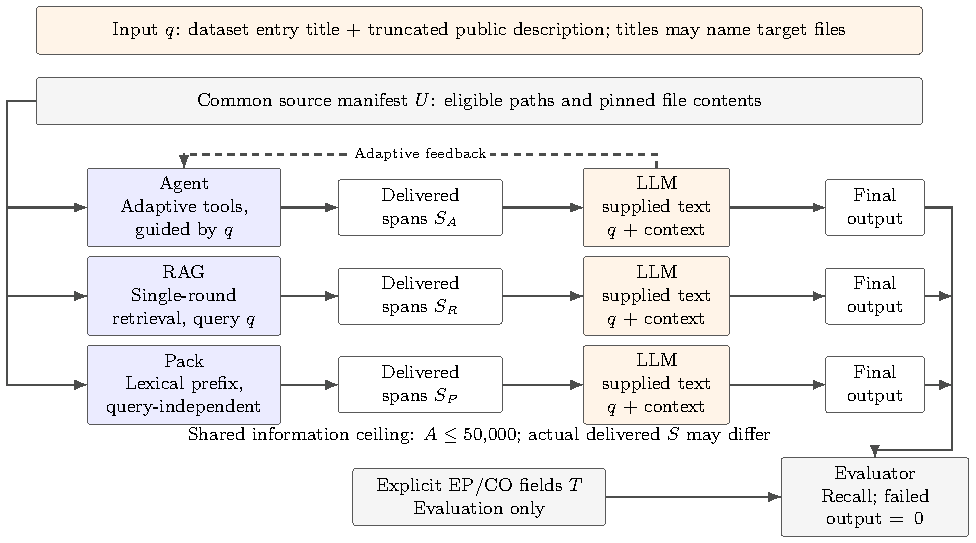
\includegraphics[width=0.94\textwidth]{figures/acquisition_design.pdf}
\caption{S1 acquisition and evaluation boundaries. The supplied entry title and public description guide Agent and RAG acquisition and enter final inference in every configuration. Explicit EP/CO fields $T$ enter evaluation only; entry titles may contain target filenames. Shared eligibility does not imply identical delivered source $S$ or valid final outputs.}
\label{fig:design}
\end{figure*}

\subsection{Acquisition Configurations}
\textbf{Pack.} Eligible relative paths are ordered lexicographically. A path list consumes at most 5,000 accounting tokens; numbered source lines are then appended in lexical file order within the remaining information budget. The renderer retains complete lines. This deterministic prefix is a low-complexity static reference, not a representative implementation of all context-packing strategies.

\textbf{RAG.} The dataset-supplied entry title and truncated public description form one retrieval query. Nonblank source is chunked into 60-line windows with 15-line overlap, without a chunk-count cap. BM25 uses lowercased alphanumeric/underscore terms. Dense retrieval uses BAAI/bge-small-en-v1.5~\cite{bge} through FastEmbed, cosine similarity, and a frozen 400-accounting-token truncation rule for chunk embedding text. The runtime ONNX and tokenizer bytes are hash-bound; its recorded ONNX snapshot is \texttt{aa8f8b0}, not asserted to be the upstream BAAI commit. The model-card sequence limit is 512 model tokens, a different tokenizer boundary from the chunk truncation rule. Query text is passed directly through \texttt{embed}, without an explicitly prepended retrieval instruction. Exact artifact hashes and current dependency behavior are indexed in Appendix~A. Reciprocal rank fusion~\cite{rrf} scores chunk $c$ as
\begin{equation}
 r(c)=\frac{1}{60+r_{\mathrm{sparse}}(c)}
      +\frac{1}{60+r_{\mathrm{dense}}(c)}.
\end{equation}
Complete sparse and dense rankings are fused; ties use sparse rank, relative path, and starting line. Selected chunks are rendered with headers and numbered lines until the ledger ceiling is reached. The model receives one acquisition pass, followed by final-answer handling.

\textbf{Agent.} Pi's native tool interface exposes only \texttt{list\_dir}, \texttt{grep}, and \texttt{read\_file}. Built-in general-purpose tools are disabled. Listings return at most 200 children. Search uses POSIX extended regular expressions, an optional file glob, at most 50 matches, and two surrounding lines. Reads return at most 400 lines. Tool-output caps are 4,000 accounting tokens for listings/search and 8,000 for reads. Search and read operations authorize paths against the manifest. The model chooses actions from the advisory and earlier results; the native loop may issue multiple calls in one assistant message.

At most 40 accepted bridge execution actions and 46 provider requests are permitted per unit. The action limit does not count every model tool attempt: Pi may reject arguments before bridge execution. Agent's stateful interaction also differs from the single context presentation used by Pack and RAG.

\subsection{Final-Answer Handling and Termination}
S1 validates the defined JSON/XML-compatible answer envelope, including positive integer line coordinates. Nonempty invalid final text receives at most one formatting correction requesting only the final JSON object. Empty final text fails directly without that correction. The native collector retains text from the last completed assistant message, excludes thinking blocks from answers, and finishes after the native loop settles. DSML tool-call text is outside the accepted final-answer forms.

When a normal bridge action reaches the action or information ceiling, the extension disables active tools. That action still returns its source or listing text plus an exhaustion flag stored in tool-result details. It does not append a new final-answer instruction at that transition. The bridge returns an explicit budget-exhausted instruction if another queued call starts with the budget already exhausted. An offline probe of the installed Pi message converter shows that tool-result details are not sent as model-visible content. Initial instructions and any later formatting correction remain distinct from this transition.

The transport has a 600-second completion-wait timeout, initially measured from prompt start and reset at each completed assistant message. It is not a 600-second total task limit and is not reset at each token. S0 instead applies a 600-second timeout to each explicit prompt. No retained effective unit exceeds 600 seconds in recorded total time (maxima: S0 531.2 seconds, S1 387.0 seconds). Interrupted infrastructure attempts are recorded separately.

\subsection{Information and Resource Accounting}
The shared repository-information ceiling is $A\leq50{,}000$. $A$ sums newly delivered blocks using \texttt{cl100k\_base}: source headers, numbered code, listings, search results, repeated acquisitions, and errors represented in the bridge ledger. Replayed conversation history is not charged again to $A$. Exact block text, token counts, hashes, and source spans are recorded.

This is a ledger of acquisition output, not all model-visible feedback. S1 contains 174 Pi argument-validation error results (173 search, one read) that bypass the bridge and enter neither $A$ nor its execution-action count. They deliver no new repository source. Consequently, the verified ceiling bounds the ledger and delivered repository content; it does not assert that every feedback token is included.

We separately measure cumulative provider input $B$, output tokens, provider-reported fees, and recorded unit time. $B$ includes instructions, advisory text, delivered blocks, replayed history, and cached input. Its tokenizer and scope differ from $A$; the two counts must not be treated as interchangeable budgets. Offline source preparation and index construction are excluded from online timing. The recorded unit window begins after initial source/index validation and some model preparation, so it is not full cold-start latency.

\section{Experimental Setup}
\label{sec:setup}
\subsection{Sample and Model}
We use the human-verified portion of VulnGym v0.1.4 at dataset commit \texttt{cd69f7e}~\cite{vulngymdata}. Excluding pilot entries and their advisories leaves 338 entries from 156 advisories. The frozen sampling procedure retains one representative per advisory and selects 80 entries plus ten reserves using seed 20260929. Reserves are not evaluated. The sample contains 60 business-logic and 20 traditional-vulnerability entries, 130 entry-specific unique EP/CO target files, and 74 canonical repository--commit pairs across 13 repositories.

The sample is concentrated: Openclaw contributes 45 entries, n8n 12, and Flowise eight; the other ten repositories contribute 15 entries. Distinct advisories do not imply independent repositories. The public description is capped at 1,500 characters with the frozen truncation marker. The pre-existing \texttt{PATH\_HINT} flag labels 29 descriptions matching a case-insensitive source-path or filename/extension pattern; the remaining 51 are \texttt{NO\_PATH\_HINT}. This flag inspects the description alone, omitting the supplied title. We retain the frozen labels and refer to them as description-only flags.

A post hoc input audit matches each EP/CO target basename as a case-insensitive substring of the archived title. At least one basename matches in 47/80 entries: 12/29 in the description-hint group and 35/51 in the other group (Table~\ref{tab:input-hints}). A match need not identify a unique repository path, and not every match is proved to originate from an appended suffix. Neither description stratum represents input free of filename hints.
% Generated by generate_input_output_diagnostics.py; see input_output_provenance.json
\begin{table*}[t]
\centering\small
\caption{Description-only hint flags and target-basename matches in supplied entry titles.}\label{tab:input-hints}
\begin{adjustbox}{max width=\textwidth}\begin{tabular}{lrr}
\toprule
Frozen description flag & Entries & Title basename matches \\
\midrule
PATH\_HINT & 29 & 12 \\
NO\_PATH\_HINT & 51 & 35 \\
\bottomrule
\end{tabular}\end{adjustbox}
\par\vspace{3pt}\begin{minipage}{\textwidth}\footnotesize Matching is case-insensitive substring matching of a target basename, not full-path matching or an estimate of hint effects. The two original flags are retained; neither defines a hint-free input group.\end{minipage}
\end{table*}


Both studies use DeepSeek V4 Pro with high reasoning effort through Pi. Pi 0.85.1, Python 3.12.3, WSL2, embedding artifacts, dependency fingerprints, configuration, command, and timestamps are recorded with the study artifacts. The client records the model setting, but does not make provider generation deterministic or verify an identical hidden backend throughout collection. Fixed schedule and analysis seeds therefore coexist with stochastic model outcomes.

\subsection{Two Separately Frozen Studies}
Each study schedules 80 entries $\times$ three configurations $\times$ three repeats, or 720 unique inference units. Every arm has 240 outcomes. Repeats are averaged within an entry before paired comparisons; they are not 240 independent statistical samples.

S0 records the original text-tool interface, renderer, parser, source filters, and capped retrieval indexes. Its Agent source predicate admits 578 additional nonblank files excluded by Pack's directory/size/binary rules. Pack and Agent permit all 130 target files; RAG's 40,000-chunk index cap excludes two, in \texttt{entry-00183} and \texttt{entry-00359}. Pack's delivered prefix contains no target-file source, despite target eligibility. This last observation is an acquisition result, not an eligibility exclusion.

S1's scientific implementation and analysis were frozen before its formal collection, after S0 outcomes and implementation issues were known. It uses the shared manifest and renderer of Section~\ref{sec:method}, full indexes totaling 2,033,973 chunks, a native Agent interface, and schedule seed 20261003. The largest snapshot contains 56,867 chunks. Table~\ref{tab:configuration-changes} records the bundled changes. They include retrieval tie/numerical details, scheduling, output validation, and timeout semantics as well as source eligibility.
% Generated by paper/generate_revision_artifacts.py; see paper/provenance.json
\begin{table*}[t]
\centering
\caption{Implementation dimensions differing between S0 and S1. The two studies use the same known sample, not a single-factor intervention.}\label{tab:configuration-changes}
\small
\begin{adjustbox}{max width=\textwidth}\begin{tabular}{p{.15\textwidth}p{.35\textwidth}p{.40\textwidth}}
\toprule
Dimension & S0 & S1 \\
\midrule
Source/index & Arm-specific filters; RAG cap of 40,000 chunks & Shared authorization; every nonblank eligible chunk indexed \\
Agent interface & Text tool JSON and explicit experiment loop & Native schemas and Pi loop; multiple calls per assistant message \\
Final parsing & JSON extracted with permissive candidate validation & Bounded envelope; at most five valid positive integer intervals \\
Presentation & Pack tree; chunk interval headers; grep matches & Eligible path listing; numbered lines; grep context \\
Retrieval ties & Stable original ordering & Explicit sparse rank, path and starting line \\
Scheduling & Entry-first schedule & Repeat-first shuffled entry/arm schedule \\
Waiting timeout & 600 seconds per explicit prompt & 600 seconds, reset after each native assistant completion \\
\bottomrule
\end{tabular}\end{adjustbox}
\par\vspace{3pt}\begin{minipage}{\textwidth}\footnotesize S0 files are bound to the original launch manifest; S1 files are bound to the archived implementation. These descriptions are implementation observations, not estimated effects of individual changes.\end{minipage}
\end{table*}


Output validity is not identical across studies. Seven accepted S0 Agent answers contain a \texttt{line\_end=null} candidate that would invalidate the entire answer under S1's schema. Applying the strict schema to saved S0 answers gives Agent FR@5 0.8188 and LR@5 0.6417, with the original full denominator. This offline sensitivity check is not a replacement for S0 scores or a simulation of generation under S1 prompts. We retain each study's frozen output policy and do not pool its observations with the other study.

\subsection{Localization Metrics}
For entry $i$, let $T_i$ contain the one or two unique EP/CO paths and $P_{ir,5}$ the paths in the first five predictions for repeat $r$. The unit file score is
\begin{equation}
 \mathrm{FR@5}_{ir}=\frac{|T_i\cap P_{ir,5}|}{|T_i|}.
\end{equation}
The reported arm mean averages the three repeats per entry and then the 80 entries. It is not a pooled proportion of the 130 target files. It measures coverage rather than precision.

The shared user instruction ends with \emph{Identify the most likely vulnerable code locations.} The system instruction requests up to five likely vulnerable files with line intervals. Neither explicitly requests separate EP and CO predictions; the returned list is undifferentiated. Accordingly, the role-based scores measure coverage of benchmark annotations, not compliance with an explicit two-role task.

LR@5 keeps a denominator of two annotations, EP and CO, even when they share a path. For annotated interval $[u,v]$, a prediction hits if its path matches and its schema-valid integer interval $[a,b]$ satisfies
\begin{equation}
 a-5\leq v\quad\text{and}\quad b+5\geq u.
\end{equation}
An annotation without a qualifying prediction contributes zero. This criterion permits interval overlap with five-line tolerance; it does not require exact lines or containment of the full annotation. For example, a same-file prediction [1,1000] hits an annotation [500,510] despite its coarse extent. The frozen S1 supplementary metric LR@5$_{\leq64}$ additionally discards predicted intervals with inclusive width $b-a+1>64$; its denominator remains two and its hit rule remains overlap-based. We report it descriptively, without adding a post hoc test family.

\subsection{Analysis and Retained Failures}
The primary contrast frozen before collection is Agent--Pack FR@5. The secondary family comprises Agent--RAG and RAG--Pack contrasts for FR@5 and LR@5. Two-sided Monte Carlo sign-flip tests use 100,000 draws and a plus-one correction. Percentile intervals use 10,000 entry-bootstrap draws; analysis seed is 20260928. The primary threshold is $p<0.05$. Four secondary tests use Benjamini--Hochberg adjustment~\cite{bh} at $q<0.10$. S0 adjusts probabilities rounded to four decimals; S1 adjusts unrounded probabilities. Original statistics are retained.

Both procedures assume independence between entry-level differences. We therefore report repository means, leave-one-repository-out aggregates, an equal-repository mean, and the frozen repository-resampling sensitivity interval. Displayed entry intervals are unadjusted for both clustering and multiplicity.

During manuscript review, we add a separate post hoc sensitivity analysis for all five frozen contrasts. It enumerates all $2^{13}=8{,}192$ sign assignments to repository sums of the repeat-averaged entry differences. This retains the entry-weighted contrast as its estimand but assumes independently sign-exchangeable repository contributions. An exploratory four-secondary-test BH adjustment is calculated separately from the frozen entry-level family. Equal-repository means instead give every repository equal weight, and leave-one-repository-out means expose concentration. These diagnostics neither replace the official tests nor provide a general cluster-robust estimator; no CR2 analysis was implemented. We describe the original description-only hint strata using every outcome. Additional post hoc diagnostics audit title basenames and jointly classify source delivery and output at the annotation level. Each arm retains 480 opportunities: two annotations in each of 240 outcomes, even when EP and CO share a path. Delivered annotation source requires an actual recorded span to overlap the annotation, with zero tolerance. Prediction hits retain the frozen five-line tolerance. Invalid output takes precedence; other opportunities are partitioned by hit/miss, target-file delivery, and annotated-source delivery (Table~\ref{tab:annotation-stages}). These categories use the union of saved delivered spans and final predictions. They measure co-occurrence, not a temporal sequence or verified evidence use. We cross-tabulate them by annotation role and retention under the frozen 64-line rule.

We also report EP and CO recall separately, predicted-interval width quantiles, and the union of predicted lines within each file. Width quantiles describe valid returned intervals; mean union extent retains all 240 outcomes, assigning zero to failures. A paired decomposition partitions the Agent--RAG score difference by whether Agent returned a valid output, keeping 240 as the denominator for both contributions. We additionally check each top-five prediction against the full pinned Git tree and the file's length. Path existence is distinct from eligibility; existing filtered files are counted separately. The original union extent is model-reported numeric range size. A clipped extent removes nonexistent paths, intersects each interval with the actual file, and then merges within each path, averaging all 240 outcomes. Neither extent measures analyst effort. These diagnostics leave frozen scores and tests unchanged and do not estimate repaired-system performance.

An empty or invalid final model output scores FR@5=LR@5=0 and remains in the denominator. Completed output failures are never retried or replaced. Explicitly authorized infrastructure recovery resumes incomplete units while retaining interrupted attempts, diagnostics, and billing status. S1's completed matrix preserves all 31 Agent output failures and all 720 scheduled keys. The complete frozen schedule, code archive, recovery ancestry, delivered blocks, and effective-outcome fee journal are bound to the analysis artifacts; historical unresolved charges remain separate.

\section{Results}
\label{sec:results}
\subsection{RQ1: Localization with the Full Denominator}
Table~\ref{tab:means} reports S0 and S1 separately. S1 FR@5 is \SOneAgentFR{} for Agent, \SOneRagFR{} for RAG, and \SOnePackFR{} for Pack. The primary Agent--Pack difference is \SOnePrimary{}, with 95\% entry-bootstrap interval \SOnePrimaryCI{} and Monte Carlo $p=1/100001$. RAG--Pack FR@5 differs by 0.3500. Both query-dependent configurations exceed the lexical-prefix reference on this sample.
% Generated by paper/generate_revision_artifacts.py; see paper/provenance.json
\begin{table}[t]
\centering
\caption{File and line localization in the two studies. Each cell averages three repeats within each of 80 entries; all failures remain in the denominator.}\label{tab:means}
\small
\begin{adjustbox}{max width=\columnwidth}\begin{tabular}{llrrr}
\toprule
Study & Configuration & FR@5 & LR@5 & Failures \\
\midrule
S0 & Agent & 0.8458 & 0.6583 & 6/240 \\
S0 & RAG & 0.7875 & 0.4917 & 0/240 \\
S0 & Pack & 0.4271 & 0.2375 & 0/240 \\
S1 & Agent & 0.7479 & 0.5813 & 31/240 \\
S1 & RAG & 0.7729 & 0.4938 & 0/240 \\
S1 & Pack & 0.4229 & 0.2500 & 0/240 \\
\bottomrule
\end{tabular}\end{adjustbox}
\par\vspace{3pt}\begin{minipage}{\columnwidth}\footnotesize S0: original configuration study. S1: supplementary study on the same known sample, with a common eligible source universe and native Agent tools. These are separate studies, not independent samples.\end{minipage}
\end{table}

% Generated by paper/generate_revision_artifacts.py; see paper/provenance.json
\begin{table*}[t]
\centering
\caption{S1 paired comparisons using the frozen analysis. Differences use the first configuration minus the second.}\label{tab:contrasts}
\small
\begin{adjustbox}{max width=\textwidth}\begin{tabular}{llrrll}
\toprule
Comparison & Role & $\Delta$ & 95\% entry-bootstrap CI & $p$ & BH $q$ \\
\midrule
Agent--Pack FR & Primary & 0.3250 & [0.2271, 0.4229] & $<0.0001$ & --- \\
Agent--RAG FR & Secondary & -0.0250 & [-0.0771, 0.0271] & 0.3970 & 0.3970 \\
Agent--RAG LR & Secondary & 0.0875 & [0.0250, 0.1521] & 0.0112 & 0.0149 \\
RAG--Pack FR & Secondary & 0.3500 & [0.2583, 0.4396] & $<0.0001$ & $<0.0001$ \\
RAG--Pack LR & Secondary & 0.2438 & [0.1604, 0.3271] & $<0.0001$ & $<0.0001$ \\
\bottomrule
\end{tabular}\end{adjustbox}
\par\vspace{3pt}\begin{minipage}{\textwidth}\footnotesize Two-sided Monte Carlo sign flips: 100,000 draws, plus-one correction. The four secondary comparisons form one BH family with the frozen threshold $q<0.10$. Intervals resample entries and are not adjusted for repository clustering or multiple comparisons.\end{minipage}
\end{table*}


The Agent--RAG file contrast is \SOneAgentRagFR{}, with interval [-0.0771, 0.0271] and $p=q=\SOneAgentRagFRP{}$. It does not meet the frozen secondary criterion. The interval allows an Agent disadvantage of 7.71 percentage points and an advantage of 2.71 points under the entry-resampling assumptions; this result does not establish equivalence. Agent--RAG LR@5 differs by \SOneAgentRagLR{}, with interval [0.0250, 0.1521] and BH $q=\SOneAgentRagLRQ{}$ under the same entry-independence assumption. RAG--Pack LR@5 differs by 0.2438 (Table~\ref{tab:contrasts}).

Table~\ref{tab:cluster-sensitivity} places these contrasts alongside the post hoc repository diagnostics. For Agent--RAG LR@5, the equal-repository mean is 0.0533, and the exact repository sign-flip probability is 0.0781, with exploratory secondary $q=0.1042$. Thus the observed 0.0875 entry-weighted difference remains a sample description, while secondary inferential support is sensitive to the dependence assumptions. RAG--Pack FR@5 also has exploratory repository $q=0.1042$, compared with 0.0059 for RAG--Pack LR@5. These probabilities are separate sensitivities, not replacements for the frozen analysis or proof of general repository-level effects.
% Generated by paper/generate_review_sensitivity.py; see review_sensitivity_provenance.json
\begin{table*}[t]
\centering\small
\caption{Post-hoc S1 repository sensitivity for all frozen contrasts.}\label{tab:cluster-sensitivity}
\begin{adjustbox}{max width=\textwidth}\begin{tabular}{lrrrrr}
\toprule
Contrast & Entry mean & Equal-repo mean & Leave-one-repo range & Repo $p$ & Repo $q$ \\
\midrule
Agent--Pack FR & 0.3250 & 0.2228 & [0.2894, 0.3377] & 0.0313 & --- \\
Agent--RAG FR & -0.0250 & 0.0209 & [-0.0463, 0.0049] & 0.6250 & 0.6250 \\
RAG--Pack FR & 0.3500 & 0.2018 & [0.3186, 0.3701] & 0.0625 & 0.1042 \\
Agent--RAG LR & 0.0875 & 0.0533 & [0.0787, 0.0952] & 0.0781 & 0.1042 \\
RAG--Pack LR & 0.2438 & 0.3943 & [0.2245, 0.3238] & 0.0015 & 0.0059 \\
\bottomrule
\end{tabular}\end{adjustbox}
\par\vspace{3pt}\begin{minipage}{\textwidth}\footnotesize Repeats are averaged within entries before grouping the 80 entries into 13 repositories. Exact two-sided sign flips enumerate all $2^{13}=8{,}192$ repository signs using sums of entry differences; this retains the entry-weighted estimand and assumes independently sign-exchangeable repository contributions. The last column is exploratory Benjamini--Hochberg correction across the four secondary comparisons. It does not replace frozen entry-level inference or provide general cluster-robust validity. Equal-repository means target a different weighting.\end{minipage}
\end{table*}


\begin{figure}[t]
\centering
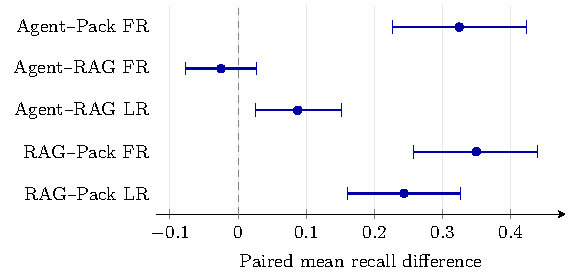
\includegraphics[width=\columnwidth]{figures/s1_contrasts.pdf}
\caption{S1 paired mean differences and 95\% entry-bootstrap intervals from the frozen analysis. FR is file coverage; LR is tolerance-based interval recall. Intervals are unadjusted and assume independent entries.}
\label{fig:contrasts}
\end{figure}

S0's Agent--Pack FR@5 difference is 0.4188, with interval [0.3333, 0.5062]. Its Agent--RAG file contrast is positive, 0.0583, with $p=q=0.0529$ under S0's secondary procedure. The latter passes S0's frozen $q<0.10$ criterion but not a per-comparison $p<0.05$ threshold. In S1 the point estimate changes sign. These observations accompany the bundled configuration changes; they are not evidence that a particular repair caused the difference.

\subsection{RQ2: Evidence Delivery and Final Output}
Table~\ref{tab:delivery} separates source acquisition from prediction. Agent delivers code from 48.0 unique paths per unit on average, RAG 51.5, and Pack 51.7. Their mean fractions of target files with any delivered source are 0.9542, 0.6813, and 0.0000. The fractions average each unit's one- or two-file target coverage; they are not pooled counts across three repeats.
% Generated by paper/generate_revision_artifacts.py; see paper/provenance.json
\begin{table}[t]
\centering
\caption{S1 descriptive context delivery and supplementary line scoring. Source files count unique paths with delivered code spans; directory and path-only listings are excluded.}\label{tab:delivery}
\small
\begin{adjustbox}{max width=\columnwidth}\begin{tabular}{lrrr}
\toprule
Configuration & Files/unit & Mean $|T\cap F(S)|/|T|$ & LR@5$_{\leq64}$ \\
\midrule
Agent & 48.0 & 0.9542 & 0.5042 \\
RAG & 51.5 & 0.6813 & 0.2729 \\
Pack & 51.7 & 0.0000 & 0.0208 \\
\bottomrule
\end{tabular}\end{adjustbox}
\par\vspace{3pt}\begin{minipage}{\columnwidth}\footnotesize Target fractions are averaged per unit, with one or two EP/CO target files per entry. The last column excludes predicted intervals longer than 64 lines; it remains an overlap-based recall measure.\end{minipage}
\end{table}


Agent's higher delivery coverage coexists with lower aggregate FR@5 than RAG. A hit in a target file can expose irrelevant lines, and a final prediction can omit an acquired target. The present summaries establish this difference between availability and output, without isolating those explanations. Pack achieves FR@5 \SOnePackFR{} despite no target-source delivery. The model still receives the advisory and path list; these and prior knowledge are possible information routes, whose individual contributions are not measured.

\subsection{Annotated Source, Returned Locations, and Prediction Extent}
The post hoc joint analysis moves from any code in a target file to overlap with its annotated interval. Mean annotation-source delivery is 0.9125 for Agent, 0.3813 for RAG, and zero for Pack, retaining all outcomes. Table~\ref{tab:annotation-stages} partitions 480 opportunities per arm. Agent has 279 credited interval hits, all accompanied by delivered annotation source. It also leaves 108 annotations uncovered in schema-valid outputs with such source available. RAG has 141 hits with annotation source and 96 without it; its uncovered annotations in schema-valid outputs divide into 102 without target-file code, 99 with only other lines from that file, and 42 with annotation-source delivery. Pack's 120 hits all occur without target-file source. Source and hit co-occurrence is an availability diagnostic; reasons and security traces are not adjudicated.
% Generated by generate_input_output_diagnostics.py; see input_output_provenance.json
\begin{table*}[t]
\centering\small
\caption{Joint annotation-level source and output outcomes in S1 (post hoc).}\label{tab:annotation-stages}
\begin{adjustbox}{max width=\textwidth}\begin{tabular}{lrrrrrr}
\toprule
Configuration & Invalid & Hit + source & Hit, no source & Miss, no file & Miss, file only & Miss + source \\
\midrule
Agent & 62 & 279 & 0 & 14 & 17 & 108 \\
RAG & 0 & 141 & 96 & 102 & 99 & 42 \\
Pack & 0 & 0 & 120 & 360 & 0 & 0 \\
\bottomrule
\end{tabular}\end{adjustbox}
\par\vspace{3pt}\begin{minipage}{\textwidth}\footnotesize Each row partitions all 480 EP/CO opportunities (240 outcomes, two annotations each). Source means exact overlap of delivered code with the annotated interval; a hit uses the frozen five-line-tolerance rule. Invalid output overrides source categories. Hit/source co-occurrence does not verify model use or rationale.\end{minipage}
\end{table*}

% Generated by generate_input_output_diagnostics.py; see input_output_provenance.json
\begin{table*}[t]
\centering\small
\caption{Annotation delivery, role recall, and predicted interval extent (post hoc).}\label{tab:interval-detail}
\begin{adjustbox}{max width=\textwidth}\begin{tabular}{lrrrrrr}
\toprule
Configuration & Annotation source & EP recall & CO recall & Width median & Width P90 & Union lines/unit \\
\midrule
Agent & 0.9125 & 0.4083 & 0.7542 & 22.0 & 75.0 & 88.4 \\
RAG & 0.3813 & 0.3750 & 0.6125 & 38.0 & 220.0 & 264.9 \\
Pack & 0.0000 & 0.2375 & 0.2625 & 200.0 & 300.0 & 629.8 \\
\bottomrule
\end{tabular}\end{adjustbox}
\par\vspace{3pt}\begin{minipage}{\textwidth}\footnotesize Annotation source is averaged over all 480 annotation opportunities. EP and CO recall each retain 240 outcomes. Width quantiles summarize intervals in valid top-five answers; union lines/unit merges overlapping predicted intervals within a file and averages all 240 outcomes, including zero lines for failures. These are model-reported numeric extents, including absent paths and out-of-bounds lines, not readable code or measured human effort.\end{minipage}
\end{table*}


% Generated by generate_review_resolution.py; see review_resolution_provenance.json
\begin{table*}[t]
\centering\small
\caption{Joint annotation coverage by role and prediction width (post hoc).}\label{tab:role-width}
\begin{adjustbox}{max width=\textwidth}\begin{tabular}{lrrrrrr}
\toprule
Configuration & Role & Source, no hit & Correct path subset & Hit, no ann. source & Retained at 64 & No file source subset \\
\midrule
Agent & EP & 80 & 53 & 0 & 0 & 0 \\
Agent & CO & 28 & 25 & 0 & 0 & 0 \\
RAG & EP & 36 & 23 & 39 & 0 & 26 \\
RAG & CO & 6 & 3 & 57 & 5 & 25 \\
Pack & EP & 0 & 0 & 57 & 4 & 57 \\
Pack & CO & 0 & 0 & 63 & 6 & 63 \\
\bottomrule
\end{tabular}\end{adjustbox}
\par\vspace{3pt}\begin{minipage}{\textwidth}\footnotesize Each role has 240 opportunities. Source/no-hit requires schema-valid output; the next column is its correct-path subset. The final two columns are subsets of hits without annotated source. Retained at 64 uses the frozen width-limited rule. Categories describe co-occurrence, not task failure or evidence use.\end{minipage}
\end{table*}

% Generated by generate_review_resolution.py; see review_resolution_provenance.json
\begin{table*}[t]
\centering\small
\caption{Repository validity of returned intervals (post hoc).}\label{tab:location-validity}
\begin{adjustbox}{max width=\textwidth}\begin{tabular}{lrrrrr}
\toprule
Configuration & Intervals & Absent path & End beyond EOF & Affected units / 240 & Clipped lines/unit \\
\midrule
Agent & 635 & 0 & 2 & 2 & 88.2 \\
RAG & 774 & 23 & 52 & 56 & 228.8 \\
Pack & 763 & 381 & 129 & 180 & 261.5 \\
\bottomrule
\end{tabular}\end{adjustbox}
\par\vspace{3pt}\begin{minipage}{\textwidth}\footnotesize Counts refer to top-five predictions. Paths are checked against the complete pinned Git tree; existing files use recorded line counts. Three Pack intervals refer to existing filtered files. Clipped extent drops absent paths, bounds intervals by file length, merges within each path, and averages all 240 outcomes including failures. These diagnostics do not rescore frozen outcomes or measure analyst effort.\end{minipage}
\end{table*}


Table~\ref{tab:role-width} clarifies the coverage categories. Of Agent's 108 uncovered annotations with source available, 80 are EP and 28 CO; 78 already have the correct file among the predictions. Two purposively selected counterexamples illustrate why this is not automatically task failure. For \texttt{entry-00227}, repeat 1, Agent returns lines 121--146 of \path{src/agents/tools/sessions-spawn-tool.ts}, covering the CO at line 129 but not the EP factory declaration at line 60. For \texttt{entry-00229}, repeat 1, its lines 253--267 of \path{src/agents/apply-patch.ts} cover the sandbox operation at CO line 258, not the EP factory at line 80. These cases demonstrate role-specific annotation omissions while a critical operation is returned; they do not validate every rationale or estimate their prevalence.

Of RAG's 96 hits without corresponding annotation source, 45 have other source from the target file and 51 have none. Only five retain a hit under the 64-line rule, all at CO; the other 91 depend on broader returned intervals. Pack retains ten of its 120 such hits. Thus hits without annotated source predominantly describe broad overlap credit in these records, rather than demonstrated precise localization without source.

Table~\ref{tab:location-validity} separates schema acceptance from repository-valid locations. RAG's 774 returned intervals contain 23 nonexistent paths and 52 intervals ending beyond the file; Pack's 763 contain 381 and 129 respectively. Agent's 635 contain no nonexistent paths and two overruns. At least one such issue occurs in 56 RAG, 180 Pack, and two Agent outcomes. For example, Pack predicts lines 1--250 of \path{packages/server/src/routes/chatflows/index.ts} in \texttt{entry-00477}, whose file contains 43 lines. After removing absent paths and clipping to file lengths, mean within-file union extents are 88.2, 228.8, and 261.5 lines per outcome for Agent, RAG, and Pack. These are descriptive location checks, not replacements for the frozen scores.


Prediction extents help interpret those hits. Across returned top-five intervals, median widths are 22 lines for Agent, 38 for RAG, and 200 for Pack; the corresponding 90th percentiles are 75, 220, and 300. Mean within-file union extents per scheduled outcome are 88.4, 264.9, and 629.8 lines, including zero for failures. These are model-reported numeric extents, including nonexistent paths and out-of-bounds lines; they do not measure readable source or analyst effort. Agent's EP and CO recalls are 0.4083 and 0.7542, versus RAG's 0.3750 and 0.6125: the larger role-specific difference is at CO.

Width-limited LR@5$_{\leq64}$ is 0.5042 for Agent, 0.2729 for RAG, and 0.0208 for Pack. Relative to ordinary LR@5, excluding broad intervals reduces Agent's score by 0.0771, RAG's by 0.2208, and Pack's by 0.2292. The difference between the line measures is consequential, especially for RAG and Pack. Agent's higher width-limited point estimate remains descriptive; no additional significance test was registered.

S1 retains 31 Agent output failures: 22 final DSML tool-call texts and nine empty final text fields. The nine empty fields arise from completed assistant messages containing thinking but no text, rather than absence of any assistant message. RAG and Pack have no schema-level output failures; location-validity issues are counted separately. All 31 Agent failures contribute zeros to the reported means.

A descriptive paired decomposition retains the denominator of 240: Agent's 209 valid-output units contribute $+0.0521$ to Agent--RAG FR@5, while its 31 invalid-output units contribute $-0.0771$, summing to $-0.0250$. For LR@5, the contributions are $+0.1229$ and $-0.0354$, summing to $+0.0875$. These are contributions to the observed contrast, not subset performance estimates or a forecast for a repaired Agent.

The native events locate an operational boundary (Table~\ref{tab:completion}). Active tools close in 53 Agent units: 36 reach 40 accepted bridge actions and 17 exhaust the information budget. Those units include 22 valid answers and all 31 failures; the other 187 units return valid answers. All 22 DSML failures receive an explicit final-JSON formatting correction and remain invalid. The nine empty outputs receive no correction. Only one failed unit receives the bridge's fixed budget-exhausted text.
% Generated by paper/generate_revision_artifacts.py; see paper/provenance.json
\begin{table}[t]
\centering
\caption{S1 Agent final-output status by observed tool-declaration closure (post-hoc).}\label{tab:completion}
\small
\begin{adjustbox}{max width=\columnwidth}\begin{tabular}{lrrrr}
\toprule
Tool state & Units & Schema-valid & DSML & Empty \\
\midrule
Never closed & 187 & 187 & 0 & 0 \\
Closed & 53 & 22 & 22 & 9 \\
\bottomrule
\end{tabular}\end{adjustbox}
\par\vspace{3pt}\begin{minipage}{\columnwidth}\footnotesize Closure follows the information or accepted-action limit. DSML denotes terminal tool-call text outside the allowed final-answer protocol. All failed units score zero. Groups are selected by an observed outcome of execution, not randomized treatments.\end{minipage}
\end{table}


\begin{figure}[t]
\centering
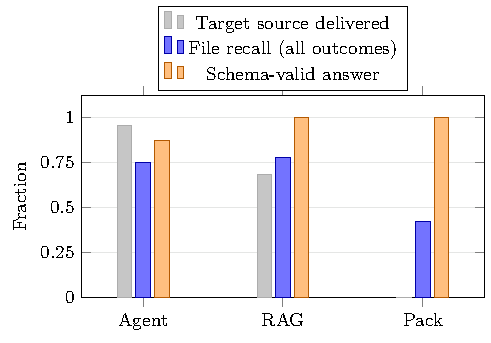
\includegraphics[width=\columnwidth]{figures/s1_delivery_output.pdf}
\caption{S1 mean target-file source coverage, FR@5, and schema-valid answer fractions across all 240 outcomes per configuration. Schema acceptance does not certify path existence, line bounds, or location correctness.}
\label{fig:delivery-output}
\end{figure}

Reviewing all saved native completion events finds no earlier usable final localization JSON overwritten in the 31 failures. Their final texts are also unrecoverable by S0's permissive parser. These observations support retaining the output failures; they do not establish that the shutdown behavior alone caused them.

\subsection{RQ3: Resources and Online Time}
Table~\ref{tab:resources} includes all 240 effective outcomes per arm, including failures. Agent's mean ledger count is 31,376 tokens, compared with approximately 50,000 for RAG and Pack. Its cumulative provider input averages 572,748 tokens, against 53,637 for RAG and 54,194 for Pack. Thus Agent uses fewer newly acquired ledger tokens but \SOneInputRatio{} times Pack's provider input. The shared acquisition ceiling does not equalize model work.
% Generated by paper/generate_revision_artifacts.py; see paper/provenance.json
\begin{table*}[t]
\centering
\caption{S1 measured resources for 240 outcomes per configuration, including model-output failures. Fees cover effective outcomes; superseded attempts are reported separately.}\label{tab:resources}
\small
\begin{adjustbox}{max width=\textwidth}\begin{tabular}{lrrrrr}
\toprule
Configuration & Mean $A$ & Mean $B$ & Fee (USD) & Mean time (s) & Median time (s) \\
\midrule
Agent & 31,376 & 572,748 & 27.154 & 107.9 & 102.8 \\
RAG & 49,996 & 53,637 & 10.120 & 58.2 & 52.9 \\
Pack & 49,994 & 54,194 & 9.970 & 52.9 & 47.2 \\
\bottomrule
\end{tabular}\end{adjustbox}
\par\vspace{3pt}\begin{minipage}{\textwidth}\footnotesize $A$: newly delivered blocks in the accounting tokenizer. $B$: cumulative provider input, including replayed history and cached input. Unit time starts after initial source/index checks and some model preparation; offline index construction and failed infrastructure attempts are outside this measure.\end{minipage}
\end{table*}


\begin{figure}[t]
\centering
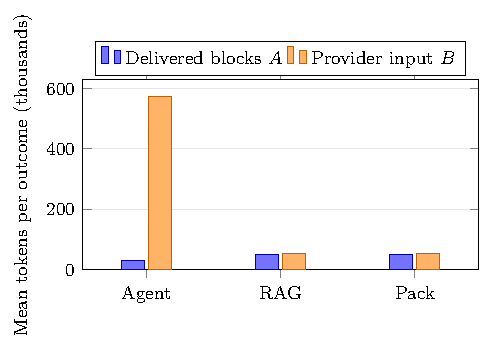
\includegraphics[width=\columnwidth]{figures/s1_input.pdf}
\caption{S1 descriptive means for newly delivered ledger information $A$ and cumulative provider input $B$. Their tokenizer and scope differ; the plot does not compare interchangeable budgets.}
\label{fig:input}
\end{figure}

Effective-outcome fees total USD \SOneFee{}. Including reported superseded attempts yields a known subtotal of USD \SOneAllFee{}, plus two historical requests whose charges remain unknown. Development calls, local compute, and index preparation are outside this subtotal. Fees are usage reports rather than independently reconciled supplier invoices.

Mean recorded unit times are 107.9 seconds for Agent, 58.2 for RAG, and 52.9 for Pack; medians are 102.8, 52.9, and 47.2 seconds. These describe the measured execution window and observed service conditions. Offline indexing is a separate investment, and initial validation/loading outside the window prevents interpreting these values as full end-to-end deployment latency.

\subsection{Sample Composition Sensitivity}
Removing any one repository leaves a positive S1 Agent--Pack aggregate contrast, ranging from \SOneLocoMin{} to \SOneLocoMax{}. The equal-repository mean is \SOneRepoEqual{}, compared with the entry-weighted \SOnePrimary{}. The frozen repository-resampling interval is [0.1500, 0.4363]. Per-repository contrasts include negatives for WeKnora and Airflow and zeros for several projects (Appendix~B). These small groups and unequal weights limit precision and generality despite a positive overall contrast. Leave-out stability does not validate the entry-independence assumption.

Table~\ref{tab:hint-subgroups} describes all S1 outcomes within the 29 description-hint and 51 description-no-match entries. Each arm has 87 and 153 outcomes respectively; Agent's four and 27 failures remain scored zero. File recall is higher in the description-hint stratum for every configuration. Pack's means are 0.7241 and 0.2516, despite no target-source delivery in either stratum. These strata differ in task and repository composition, and the latter still includes 35 titles matching target basenames. Their score difference describes the frozen description flags rather than the effect of input hints.
% Generated by paper/generate_review_sensitivity.py; see review_sensitivity_provenance.json
\begin{table*}[t]
\centering\small
\caption{S1 descriptive outcomes by the frozen description-only hint flag.}\label{tab:hint-subgroups}
\begin{adjustbox}{max width=\textwidth}\begin{tabular}{lrlrrr}
\toprule
Advisory label & Entries & Configuration & FR@5 & LR@5 & Failed \\
\midrule
PATH\_HINT & 29 & Agent & 0.8448 & 0.6034 & 4/87 \\
PATH\_HINT & 29 & RAG & 0.8621 & 0.6207 & 0/87 \\
PATH\_HINT & 29 & Pack & 0.7241 & 0.4080 & 0/87 \\
NO\_PATH\_HINT & 51 & Agent & 0.6928 & 0.5686 & 27/153 \\
NO\_PATH\_HINT & 51 & RAG & 0.7222 & 0.4216 & 0/153 \\
NO\_PATH\_HINT & 51 & Pack & 0.2516 & 0.1601 & 0/153 \\
\bottomrule
\end{tabular}\end{adjustbox}
\par\vspace{3pt}\begin{minipage}{\textwidth}\footnotesize All outcomes, including failed final answers, remain in each subgroup denominator. Labels are from the original frozen annotation rule. This is an observational subgroup description without new significance tests, a masking intervention, or contamination detection.\end{minipage}
\end{table*}


For an input-provenance example, \texttt{entry-00383} is the first evaluated entry in the frozen manifest. Its dataset title ends in \texttt{request-policy.ts}, matching target \path{src/browser/request-policy.ts}; the original title of \href{https://github.com/advisories/GHSA-xp9r-prpg-373r}{GHSA-XP9R-PRPG-373R} has no filename suffix. Its truncated description is flagged \texttt{NO\_PATH\_HINT}. This title reached all three configurations, illustrating why the description-only label cannot identify a hint-free task. Selection follows manifest order rather than scores.

\section{Discussion}
\subsection{Evidence Delivery and Localization Output}
The joint diagnostics change how aggregate scores should be read. Agent's high annotated-source coverage does not entail coverage of every benchmark role: 80 of its 108 uncovered annotations with source available are EPs, whereas the prompt requests likely vulnerable locations without separately requiring EP and CO. The two counterexamples show why an uncovered entry definition cannot automatically be attributed to failed vulnerability reasoning. Evaluations that require complete entry-to-operation coverage should state that task explicitly.

For RAG, 91 of 96 hits without annotated-source delivery disappear under the width-limited rule. This makes prediction extent central to interpreting apparent localization without source. Titles, descriptions, other code, and model knowledge remain possible information routes; the saved outcomes do not identify their individual contributions. The annotation partition is therefore a joint coverage description, not a causal chain from evidence acquisition to reasoning success.

Schema validity provides another distinct measurement. A syntactically accepted location can name a nonexistent file or exceed its length. The clipped extent makes the returned range interpretable as repository lines while preserving all outcomes, but does not measure actual analyst time. Agent's narrower ranges and higher CO recall describe its returned locations; assessing their practical usefulness also requires checking explanations and task-specific review needs.

\subsection{Completion Is Part of the Measured Configuration}
The full-denominator decomposition quantifies the completion contribution: valid Agent-output pairs contribute positively to the file contrast, but failed pairs contribute a larger negative amount. The observed ordering therefore depends materially on final-output reliability. Keeping both contributions on the original denominator exposes that dependency without selecting a favorable subset as a replacement result.

All 31 Agent failures follow closure of native tool declarations, and 22 valid answers also follow closure. On normal budget exhaustion the implementation disables tools without adding a new model-visible final instruction. Every terminal DSML failure persists after a later JSON correction; empty outputs receive no correction. These observations identify a protocol boundary worthy of intervention, while task difficulty and provider/adapter behavior remain alternative explanations. Estimating performance under a changed completion protocol requires a separately frozen intervention on an appropriately defined sample, including successful exhausted trajectories.

\subsection{Interpreting the Baselines and Budgets}
The frozen Agent--Pack primary contrast measures a query-dependent configuration against a weak lexical prefix. We retain it as registered, while Agent--RAG and the joint coverage diagnostics supply the more informative comparison. Pack describes the limitations of lexical ordering on these snapshots; structural neighborhoods, summaries, or query-driven packing would be different comparators.

Agent's smaller acquisition ledger accompanies much larger cumulative provider input. History replay increases input without delivering new source. The shared ceiling therefore defines one acquisition operating point, with measured recall, output reliability, expense, and time. Matching cumulative input or scanning acquisition limits would address different resource questions. Offline index preparation remains an additional investment for RAG.

\subsection{What the Supplementary Study Establishes}
S1 supplies a shared nonblank candidate universe on the known sample while jointly changing rendering, interaction, schema, ranking details, scheduling, and timing. Its differences from S0 describe those complete configurations. Both studies used dataset-supplied entry titles, so their numbers belong to the title-assisted setting; performance after removing annotation-added title information remains unmeasured.

The empirical contribution is the combination of these distinctions in an inspectable same-model comparison: source-rich outputs can omit an unrequested annotation role, low-source tolerant hits can depend on broad intervals, and schema-valid outputs can contain unusable coordinates. These results explain why source coverage, annotation recall, width, and location validity should be reported together for this task. They characterize the measured configurations without establishing a general ranking of acquisition policies.

\section{Threats to Validity}
\textbf{Internal validity.} S1 shares advisory inputs, model setting, nonblank source eligibility, evaluation, and acquisition ceiling. Policy-specific prompts, interaction, actual acquired information, and cumulative input remain different. Native completion behavior and empty-answer handling are part of Agent's configuration. Association between exhaustion and failure is not causal evidence. S0 additionally has eligibility/index-cap asymmetries; S1 bundles multiple changes after inspecting S0 and reuses its sample. The study estimates configuration differences and does not isolate the effect of an acquisition policy or repair.

\textbf{Construct validity.} The task uses dataset-supplied entry titles alongside public descriptions. Entry titles can contain annotation-added filenames; 47 titles match at least one target basename. Explicit label-field withholding does not remove this semantic information. All configurations share it, so it changes task difficulty and interpretation rather than candidate-universe fairness. The description-only flags cannot identify hint-free inputs. Basename matching need not be unique, and its association with scores would not estimate removal effects. Public-code training overlap is unmeasured. FR@5 measures unique target-file coverage and ignores false positives. LR@5 rewards tolerant interval overlap, while LR@5$_{\leq64}$ only limits interval width. Neither validates a complete EP--CO trace, explanation, exploit, or discovery of an unknown defect. The prompt does not separately request EP and CO, so role recall measures annotation coverage rather than full task compliance. Schema validation checks integer coordinates but not file existence or bounds; the additional location checks are descriptive. Trajectory-wide source unions do not identify when or how the model used evidence. Human-verified benchmark labels were not independently reannotated in this study. Pack's weak lexical prefix limits the meaning of comparisons against it.

\textbf{Statistical validity.} The 80 entries have distinct advisories but are clustered in 13 repositories with substantial imbalance: 45 entries come from Openclaw. Entry-level sign flips and bootstrap intervals assume independent differences and may understate uncertainty if within-repository outcomes are correlated. The post hoc repository sign-flip sensitivity also needs independent, sign-exchangeable repository contributions. Its separately adjusted secondary probabilities illustrate dependence sensitivity without certifying a general population effect. The 13 uneven clusters support limited-precision diagnostics; leave-out and repository-resampling summaries do not establish cluster-robust validity. Official secondary probabilities follow the frozen four-test BH rule; intervals are unadjusted. S0 and S1 are not pooled, and a nonsignificant contrast is not interpreted as equivalence.

\textbf{External validity.} Findings concern one hosted model, one information ceiling, a selected verified subset with dataset-title assistance, and three specific implementations. Transfer to original-advisory inputs without these title additions is unknown. Three repeats describe observed variability without controlling the provider's random generation or hidden backend. A more capable Pack, iterative RAG, other agent scaffolds, independent advisories, and additional models may differ. S1's known sample limits its use as external confirmation.

\textbf{Measurement and provenance.} The source ledger excludes Pi argument-validation feedback and provider history replay. $A$ and $B$ use different accounting scopes/tokenizers. Online time excludes initial validation and some loading, while local indexing has no complete amortized cost estimate. Reported charges depend on usage/cache accounting; two historical charges remain unresolved. The saved Pi events expose final model behavior but not complete historical HTTP bytes or an immutable archive of the whole SDK. Attribution between provider and adapter therefore remains unresolved. Source/record/hash consistency establishes an inspectable evidence chain within these boundaries, not absence of every implementation defect.

\section{Conclusion}
We compared adaptive exploration, single-round hybrid retrieval, and lexical packing for known-vulnerability localization using public descriptions and dataset-supplied entry titles. Those titles can contain target filenames, which defines the scope of the reported results. S1 shares nonblank source eligibility and retains every scheduled outcome.

Agent delivers substantially more annotated source and returns narrower intervals than RAG, but its complete-denominator file recall is lower by 2.5 percentage points. The joint analysis qualifies these outcomes: uncovered annotations with source available are predominantly entry points; most RAG hits without annotated source depend on broad intervals; and schema acceptance does not guarantee repository-valid coordinates. Agent's 31 failures contribute a negative 7.71 percentage points to the file contrast, offsetting the positive contribution from its other paired outcomes. Its higher tolerance-based line recall accompanies much greater cumulative input, with statistical support sensitive to repository dependence.

The comparison measures source acquisition, annotation coverage, interval extent, output validity, and inference expense in these configurations. Reporting S0 and S1 separately preserves the observed comparison change. The available evidence supports this joint diagnosis within the title-assisted task and the known, imbalanced sample.

\bibliographystyle{IEEEtran}
\bibliography{references}
\appendices
\section{Study Identity and Reproduction}
The public-candidate guide, \path{paper/ARTIFACT_GUIDE.md}, supplies the offline L1 commands included with this candidate. Its candidate index, \path{paper/artifact_manifest.json}, binds only the files distributed in this candidate; the historical 74-repository identity index, raw event records, fee journals, and recovery ancestry are not included in this candidate. The short study identifiers used throughout this paper map to:\\
\textbf{S0:} \path{c06-confirmatory-20261001T141449Z-4dad}\\
\textbf{S1:} \path{c06-recovery-v3-formal-20261005T142520Z-56b7}.

The raw implementation archives are authoritative for executed scientific code. Presentation and post hoc sensitivity generators bind their inputs and outputs separately; the claim--evidence map distinguishes external facts, measured observations, and untested interpretations. These materials are currently internal, with no public artifact URL. Stored analyses can be recomputed without model collection. A complete historical SDK dependency archive and provider wire transcript are unavailable, so identical future provider behavior or full historical SDK reconstruction is not certified. Recorded embedding runtime versions and ONNX/tokenizer byte hashes have a narrower, explicit scope in the guide.

S1 imports 439 completed outcomes from its immediate parent, with nested imports of 184 and 125 from earlier runs. These are overlapping ancestry counts, not additional independent observations. Completed model failures are retained. Only three unfinished infrastructure units are explicitly resumed across that chain: \texttt{entry-00117/agent/1}, \texttt{entry-00146/agent/1}, and \texttt{entry-00359/rag/2}. Original interrupted attempts remain archived. All effective-outcome requests have closed usage records; two historical charges remain unresolved rather than assigned zero.

\section{Repository Sensitivity}
% Generated by paper/generate_revision_artifacts.py; see paper/provenance.json
\begin{table}[t]
\centering
\caption{S1 repository sensitivity for the primary Agent--Pack file comparison (descriptive).}\label{tab:repos}
\small
\begin{adjustbox}{max width=\columnwidth}\begin{tabular}{lrrr}
\toprule
Repository & Entries & $\Delta$ FR & Leave-out $\Delta$ \\
\midrule
litellm & 1 & 0.0000 & 0.3291 \\
Flowise & 8 & 0.6458 & 0.2894 \\
NeMo & 1 & 0.5000 & 0.3228 \\
WeKnora & 1 & -0.1667 & 0.3312 \\
airflow & 2 & -0.0833 & 0.3355 \\
n8n-mcp & 1 & 0.0000 & 0.3291 \\
langflow & 2 & 0.0000 & 0.3333 \\
milvus & 1 & 1.0000 & 0.3165 \\
mlflow & 2 & 0.3333 & 0.3248 \\
n8n & 12 & 0.3333 & 0.3235 \\
open-webui & 1 & 0.0000 & 0.3291 \\
openclaw & 45 & 0.3333 & 0.3143 \\
paperclip & 3 & 0.0000 & 0.3377 \\
\bottomrule
\end{tabular}\end{adjustbox}
\par\vspace{3pt}\begin{minipage}{\columnwidth}\footnotesize Unequal repository sizes affect the aggregate. Per-repository estimates from one or two entries have limited precision.\end{minipage}
\end{table}

Table~\ref{tab:repos} retains all 13 repository groups, including negative and zero contrasts. The equal-repository mean differs from the entry-weighted primary estimand because repositories contribute unequal numbers of entries. The frozen repository-resampling interval is [0.1500, 0.4363]; it is a sensitivity summary from few imbalanced clusters. Neither that interval nor leave-out stability certifies independent entries.

\end{document}
